% ------------------------------------------------------------------------------
% TYPO3 v9 LTS - What's New (German Version)
%
% @license	Creative Commons BY-NC-SA 3.0
% @link		https://typo3.org/help/documentation/whats-new/
% @language	German
% ------------------------------------------------------------------------------

\section{Privacy and Security}
\begin{frame}[fragile]
	\frametitle{Datenschutz und Sicherheit}

	\begin{center}\huge{\color{typo3darkgrey}\textbf{Datenschutz und Sicherheit}}\end{center}
	\begin{center}\large{\textit{General Data Protection Regulation (GDPR) and more...}}\end{center}

\end{frame}

% ------------------------------------------------------------------------------
% General Data Protection Regulation

\begin{frame}[fragile]
	\frametitle{Datenschutz und Sicherheit}
	\framesubtitle{IP-Adressen anonymisieren}

	\begin{itemize}
		\item Ein Scheduler-Task kann aktiviert werden, um IP-Addressen in mehreren Datenbanktabellen
			nach einer bestimmten Zeitspanne zu anonymisieren
		\item Zum Beispiel die Tabelle \texttt{sys\_log}, nach 30 Tagen:
			\begin{figure}
				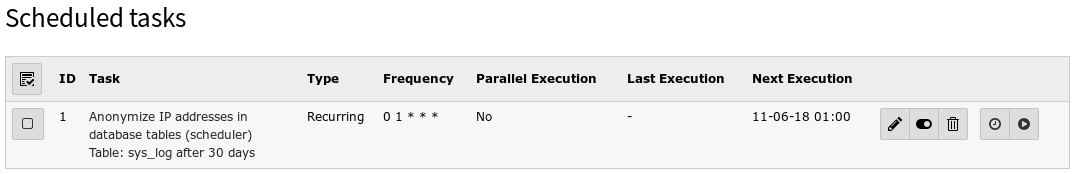
\includegraphics[width=1\linewidth]{PrivacyAndSecurity/IpAnonymizationSchedulerTask.png}
			\end{figure}
		\item Weitere Infos zur DSGVO finden Sie auf dem \href{https://typo3.com/blog/tag/gdpr/}{TYPO3 GmbH Blog}
	\end{itemize}

\end{frame}

% ------------------------------------------------------------------------------
% FE/BE User Accounts and Passwords
% #85026 - salted passwords changes

\begin{frame}[fragile]
	\frametitle{Datenschutz und Sicherheit}
	\framesubtitle{FE/BE Benutzerkonten und Passwörter}

	% decrease font size for code listing
	\lstset{basicstyle=\tiny\ttfamily}

	\begin{itemize}
		\item Unverschlüsselte Passwörter sind für BE / FE-Benutzer überhaupt nicht mehr möglich
		\item Inaktive FE/BE Benutzerdatensätze können aus der Datenbank entfernt werden, 
			indem der Schedular-Task "Table garbage collection task" hinzugefügt wird und
			"Clean all available tables" aktiviert wird\newline
			\smaller

\begin{lstlisting}
<?php
$tableGarbageCollectionTask = \TYPO3\CMS\Scheduler\Task\TableGarbageCollectionTask::class;
$GLOBALS['TYPO3_CONF_VARS']['SC_OPTIONS']['scheduler']['tasks'][$tableGarbageCollectionTask]
  ['options']['tables'] = [
  'be_users' => [
    'dateField' => 'lastlogin',
    'expirePeriod' => 30
  ]
];
\end{lstlisting}

		\item Siehe die \href{https://docs.typo3.org/typo3cms/extensions/scheduler/Installation/BaseTasks/Index.html}{Dokumentation} für weitere Infos
	\end{itemize}

\end{frame}

% ------------------------------------------------------------------------------
% #84843 - Use no-cookie domain for youtube by default

\begin{frame}[fragile]
	\frametitle{Datenschutz und Sicherheit}
	\framesubtitle{No-Cookie-Domain für Youtube-Videos}

	% decrease font size for code listing
	\lstset{basicstyle=\tiny\ttfamily}

	\begin{itemize}
		\item YouTube Videos werden standardmäßig über die No-Cookie-Domain
			\url{https://www.youtube-nocookie.com} gerendert
		\item Die reguläre Domain \texttt{www.youtube.com} kann bei Bedarf
			durch folgende TypoScript-Konfiguration erzwungen werden:

\begin{lstlisting}
lib.contentElement {
  settings {
    media {
      additionalConfig {
        no-cookie = 0
      }
    }
  }
}
\end{lstlisting}

	\end{itemize}

\end{frame}

% ------------------------------------------------------------------------------
% Password Hashing API

\begin{frame}[fragile]
	\frametitle{Datenschutz und Sicherheit}
	\framesubtitle{Password Hashing API}

	\begin{itemize}
		\item TYPO3 unterstützt nun
			\href{https://secure.php.net/manual/en/ref.password.php}{PHP Password Hashing API}.
			Dies führt 
			\href{https://en.wikipedia.org/wiki/Argon2}{Argon2i}
			und
			\href{https://en.wikipedia.org/wiki/PBKDF2}{PBKDF2} ein
	\end{itemize}

	\begin{figure}
		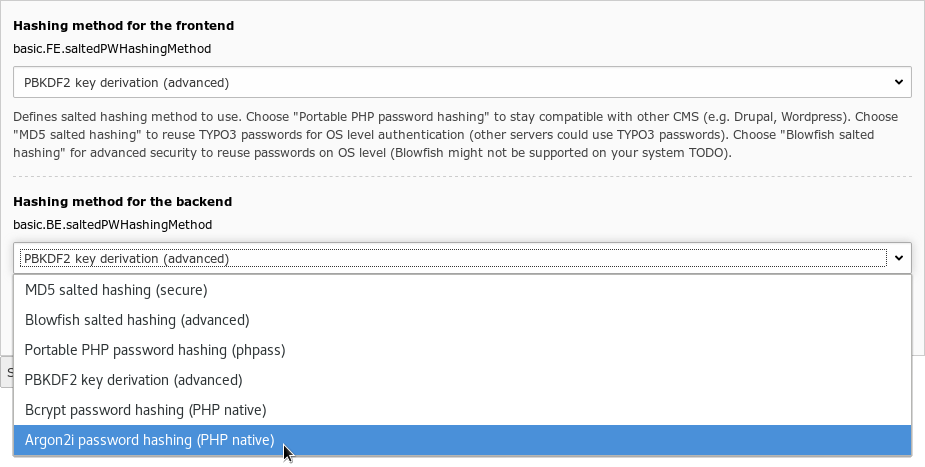
\includegraphics[width=0.7\linewidth]{PrivacyAndSecurity/PasswordHashingAlgorithms.png}
	\end{figure}

\end{frame}

% ------------------------------------------------------------------------------
% Password Hashing API

\begin{frame}[fragile]
	\frametitle{Datenschutz und Sicherheit}
	\framesubtitle{Password Hashing API}

	\begin{itemize}
		\item Integratoren können zwischen mehreren Passwort-Hashing-Methoden 
			für FE- und für BE-Passwörter wählen
		\item Angesichts der Tatsache, dass MD5 heute als sehr unsicher gilt, 
			wurde die Unterstützung von MD5-Hashes gestrichen, um Passwörter zu schützen
		\item Falls erforderlich, werden Passwort-Hashes automatisch aktualisiert, wenn sich
			Benutzer anmelden
	\end{itemize}

\end{frame}

% ------------------------------------------------------------------------------
